
%(BEGIN_QUESTION)
% Copyright 2011, Tony R. Kuphaldt, released under the Creative Commons Attribution License (v 1.0)
% This means you may do almost anything with this work of mine, so long as you give me proper credit

An operator reports a problem with the oily water filter instrumentation in this process: PDIR-136 indicates a differential pressure of 1.8 PSID, while PG-417 reads 12.5 PSI and PG-421 reads 11.3 PSI.  Your first test is to check the indication of PIR-137, and you see that it reads 12.6 PSI:

$$\includegraphics[width=15.5cm]{i0005rx01.eps}$$

Identify the likelihood of each specified fault in this process.  Consider each fault one at a time (i.e. no coincidental faults), determining whether or not each fault could independently account for {\it all} measurements and symptoms in this process.

% No blank lines allowed between lines of an \halign structure!
% I use comments (%) instead, so that TeX doesn't choke.

$$\vbox{\offinterlineskip
\halign{\strut
\vrule \quad\hfil # \ \hfil & 
\vrule \quad\hfil # \ \hfil & 
\vrule \quad\hfil # \ \hfil \vrule \cr
\noalign{\hrule}
%
% First row
{\bf Fault} & {\bf Possible} & {\bf Impossible} \cr
%
\noalign{\hrule}
%
% Another row
Upstream filter block valve partially shut &  &  \cr
%
\noalign{\hrule}
%
% Another row
Downstream filter block valve partially shut &  &  \cr
%
\noalign{\hrule}
%
% Another row
PDT-136 calibration error &  &  \cr
%
\noalign{\hrule}
%
% Another row
PT-137 calibration error &  &  \cr
%
\noalign{\hrule}
%
% Another row
PG-417 calibration error &  &  \cr
%
\noalign{\hrule}
%
% Another row
PG-421 calibration error &  &  \cr
%
\noalign{\hrule}
%
% Another row
Filter drain valve to sump left open &  &  \cr
%
\noalign{\hrule}
} % End of \halign 
}$$ % End of \vbox

Explain why the idea to check PIR-137 was a good first diagnostic test.

\vskip 20pt \vbox{\hrule \hbox{\strut \vrule{} {\bf Suggestions for Socratic discussion} \vrule} \hrule}

\begin{itemize}
\item{} Identify which fundamental principles of science, technology, and/or math apply to each step of your solution to this problem.  In other words, be prepared to explain the reason(s) ``why'' for every step of your solution, rather than merely describing those steps.
\item{} Identify the next diagnostic step you would take to isolate the problem in this system.
\item{} Identify which port on each differential pressure indicator is the ``high'' and which is the ``low'', explaining your rationale.
\item{} Estimate the amount of force applied to the 30-inch diameter manway cover on the sump by the $-2$ "WC vacuum produced by the eductor.
\end{itemize}

\underbar{file i03511}
%(END_QUESTION)





%(BEGIN_ANSWER)

\noindent
{\bf Partial answer:}

% No blank lines allowed between lines of an \halign structure!
% I use comments (%) instead, so that TeX doesn't choke.

$$\vbox{\offinterlineskip
\halign{\strut
\vrule \quad\hfil # \ \hfil & 
\vrule \quad\hfil # \ \hfil & 
\vrule \quad\hfil # \ \hfil \vrule \cr
\noalign{\hrule}
%
% First row
{\bf Fault} & {\bf Possible} & {\bf Impossible} \cr
%
\noalign{\hrule}
%
% Another row
Upstream filter block valve partially shut &  &  \cr
%
\noalign{\hrule}
%
% Another row
Downstream filter block valve partially shut &  & $\surd$ \cr
%
\noalign{\hrule}
%
% Another row
PDT-136 calibration error &  &  \cr
%
\noalign{\hrule}
%
% Another row
PT-137 calibration error &  &  \cr
%
\noalign{\hrule}
%
% Another row
PG-417 calibration error &  & $\surd$ \cr
%
\noalign{\hrule}
%
% Another row
PG-421 calibration error &  & \cr
%
\noalign{\hrule}
%
% Another row
Filter drain valve to sump left open &  & $\surd$ \cr
%
\noalign{\hrule}
} % End of \halign 
}$$ % End of \vbox


%(END_ANSWER)





%(BEGIN_NOTES)

% No blank lines allowed between lines of an \halign structure!
% I use comments (%) instead, so that TeX doesn't choke.

$$\vbox{\offinterlineskip
\halign{\strut
\vrule \quad\hfil # \ \hfil & 
\vrule \quad\hfil # \ \hfil & 
\vrule \quad\hfil # \ \hfil \vrule \cr
\noalign{\hrule}
%
% First row
{\bf Fault} & {\bf Possible} & {\bf Impossible} \cr
%
\noalign{\hrule}
%
% Another row
Upstream filter block valve partially shut &  & $\surd$ \cr
%
\noalign{\hrule}
%
% Another row
Downstream filter block valve partially shut &  & $\surd$ \cr
%
\noalign{\hrule}
%
% Another row
PDT-136 calibration error & $\surd$ &  \cr
%
\noalign{\hrule}
%
% Another row
PT-137 calibration error &  & $\surd$ \cr
%
\noalign{\hrule}
%
% Another row
PG-417 calibration error &  & $\surd$ \cr
%
\noalign{\hrule}
%
% Another row
PG-421 calibration error & $\surd$ & \cr
%
\noalign{\hrule}
%
% Another row
Filter drain valve to sump left open &  & $\surd$ \cr
%
\noalign{\hrule}
} % End of \halign 
}$$ % End of \vbox






First, the difference between the readings of PG-417 and PG-421 is 12.5 $-$ 11.3 = 1.2 PSI, which is less than the differential indicated by PDIR-136 (1.8 PSI).  The question is whether the gauges are reading incorrectly or the differential pressure transmitter is reading incorrectly.

\vskip 10pt

The fact that PIR-137 reads almost the same pressure as PG-417 suggests there is no problem with either of these instruments.  Although there is indeed a difference between these two instruments' readings, it is not sufficient to account for the discrepancy with PDIR-136.  Therefore, the problem must lie with the downstream gauge (PG-421) or the DP transmitter (PDT-136).

\vskip 10pt

The step to check PIR-137 was a good one because it validated the measurement given by PG-417, allowing us to eliminate PG-417 as a potential problem.





\vskip 20pt \vbox{\hrule \hbox{\strut \vrule{} {\bf Virtual Troubleshooting} \vrule} \hrule}

This question is a good candidate for a ``Virtual Troubleshooting'' exercise.  Presenting the diagram to students, you first imagine in your own mind a particular fault in the system.  Then, you present one or more symptoms of that fault (something noticeable by an operator or other user of the system).  Students then propose various diagnostic tests to perform on this system to identify the nature and location of the fault, as though they were technicians trying to troubleshoot the problem.  Your job is to tell them what the result(s) would be for each of the proposed diagnostic tests, documenting those results where all the students can see.

During and after the exercise, it is good to ask students follow-up questions such as:

\begin{itemize}
\item{} What does the result of the last diagnostic test tell you about the fault?
\item{} Suppose the results of the last diagnostic test were different.  What then would that result tell you about the fault?
\item{} Is the last diagnostic test the best one we could do?
\item{} What would be the ideal order of tests, to diagnose the problem in as few steps as possible?
\end{itemize}

%INDEX% Measurement, pressure: troubleshooting
%INDEX% Process: oily water sump (realistic P&ID shown)

%(END_NOTES)

